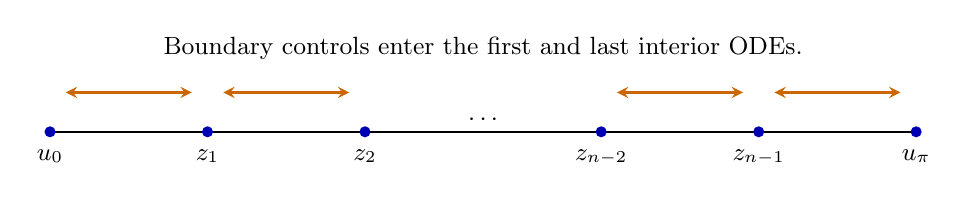
\begin{tikzpicture}[>=stealth,font=\small]
\draw[black,thick](0,0)--(11,0);
\foreach \x/\lab in {0/u_0,2/z_1,4/z_2,7/z_{n-2},9/z_{n-1},11/u_\pi}{
\fill[blue!70!black](\x,0)circle(2pt);\node[below]at(\x,-.1){$\lab$};}
\draw[<->,orange!80!black,thick](.2,.5)--(1.8,.5);
\draw[<->,orange!80!black,thick](2.2,.5)--(3.8,.5);
\draw[<->,orange!80!black,thick](7.2,.5)--(8.8,.5);
\draw[<->,orange!80!black,thick](9.2,.5)--(10.8,.5);
\node at(5.5,.15){$\cdots$};
\node[above,align=center]at(5.5,.8){Boundary controls enter the first and last interior ODEs.};
\end{tikzpicture}
